\documentclass[]{standalone}

%\usepackage{mathptmx}
%\renewcommand{\familydefault}{\rmdefault}
%\usepackage[T1]{fontenc}
%\usepackage[latin9]{inputenc}
\usepackage{siunitx}
\usepackage{array}
\usepackage{amsmath}
\usepackage{ifthen}
\usepackage{pgfplots}
\pgfplotsset{compat=1.14}
\usepackage{titling, graphicx}
\usepackage{tikz}
\usepackage{upgreek}
\usepackage{amsmath,amsthm}
\usepackage{strtikz}
\usepackage{circledsteps}
\usetikzlibrary{shapes,arrows.meta,intersections,graphs,graphs.standard}
\usetikzlibrary{bending, math,fit}
\usetikzlibrary{calc,intersections,through,backgrounds}
\usetikzlibrary{decorations.markings,decorations.pathmorphing, decorations.pathreplacing}
\usetikzlibrary{patterns}



\begin{document}



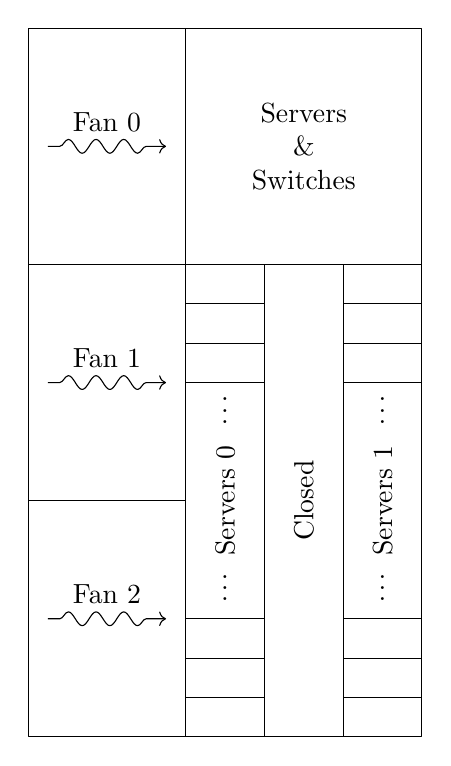
\begin{tikzpicture}[line join=round]

\draw (0,0) rectangle (5,9);

\draw (2,0) -- +(0,9);

\draw (0,3) -- +(2,0);
\draw (0,6) -- +(5,0);

\draw (3,0) -- +(0,6);
\draw (4,0) -- +(0,6);

\draw (2, 5.5) -- +(1, 0);
\draw (2, 5.0) -- +(1, 0);
\draw (2, 4.5) -- +(1, 0);
\node (dots) at (2.5, 4.25) [] {\vdots};

\draw (2, 0.5) -- +(1,0);
\draw (2, 1.0) -- +(1,0);
\draw (2, 1.5) -- +(1,0);
\node (dots) at (2.5, 2) [] {\vdots};

\draw (4, 5.5) -- +(1,0);
\draw (4, 5) -- +(1,0);
\draw (4, 4.5) -- +(1,0);
\node (dots) at (4.5,4.25) [] {\vdots};

\draw (4, 0.5) -- +(1,0);
\draw (4, 1.0) -- +(1,0);
\draw (4, 1.5) -- +(1,0);
\node (dots) at (4.5, 2) [] {\vdots};


\draw[->, decorate,decoration={snake, post length=0.15cm, pre length=0.15cm} ]
(0.25,7.5) --  node[above=2pt] {Fan 0} +(1.5,0);
\draw[->, decorate,decoration={snake, post length=0.15cm, pre length=0.15cm} ]
(0.25,4.5) --  node[above=2pt] {Fan 1} +(1.5,0);
\draw[->, decorate,decoration={snake, post length=0.15cm, pre length=0.15cm} ]
(0.25,1.5) --  node[above=2pt] {Fan 2} +(1.5,0);

\node (servers0) at (2.5, 3.0) [align=center, rotate=90] {Servers 0};
\node (servers1) at (4.5, 3.0) [align=center, rotate=90] {Servers 1};
\node (aisle) at (3.5, 3.0) [align=center, rotate=90] {Closed};

\node (servers3) at (3.5, 7.5) [align=center] {Servers\\ \& \\Switches};

\end{tikzpicture}




\end{document}
